
\documentclass{article}

\usepackage[ngerman]{babel}                     %for german umlauts
\usepackage[utf8]{inputenc}
\usepackage{subfigure}
\usepackage{float}
%\usepackage[framed,autolinebreaks,useliterate]{mcode}
%\usepackage[bw,framed,autolinebreaks,useliterate]{mcode}
% \usepackage[ansinew]{inputenc}        %for german umlauts

\usepackage{listings}

\usepackage{graphicx}
\usepackage{hyperref}

\usepackage{amssymb}    %for different fonts
\usepackage{amsmath}
% Geht nicht: \usepackage{bbm}
% \usepackage[usenames,dvips]{color} %only way to get it running with pdf:(
% \usepackage[pdftex,usenames,dvipsnames]{color}        % does not work
% \usepackage{color}
\usepackage{verbatim}
\usepackage{polynom}

\setlength{\parindent}{0pt}
\addtolength{\hoffset}{-2cm}
\addtolength{\voffset}{-1cm}
\addtolength{\textheight}{3cm}
\addtolength{\textwidth}{3cm}

\newcommand{\im}{\operatorname{Im}}
\newcommand{\rg}{\operatorname{rg}}
\newcommand{\ggt}{\operatorname{ggT}}

\lstset{ %
  language=Matlab,                % the language of the code
  frame=single,                   % adds a frame around the code
  tabsize=2,
  basicstyle=\footnotesize
}

\begin{document}

\section*{\begin{center} Mustererkennung - Aufgabenblatt 09 \end{center}}
\begin{center}
  André Hacker und Dimitri Schachmann \\
\end{center}

\subsection*{2. AdaBoost}
Wir haben für das Weihnachtsübungsblatt vor allem Aufgabe 2 bearbeitet
und dafür eine Ausprägung des AdaBoost Algorithmus implementiert. 

\verbatiminput{adaboost.m}

Bei der Auswertung haben wir festgestellt, dass wir ein anderes
Ergebnis bekommen haben, als erwartet. Wir konnten nicht beobachten,
dass der Algorithmus zuverlässig Tangenten zum Kreis auswählt. Dies
ist nämlich stark von dem Verhältnis des Kreisradius zur Bildgröße
abhängig. So konnten wir allgemein nur dann Tangenten beobachten, wenn
der Kreis an den Bildrand gestoßen ist:\\

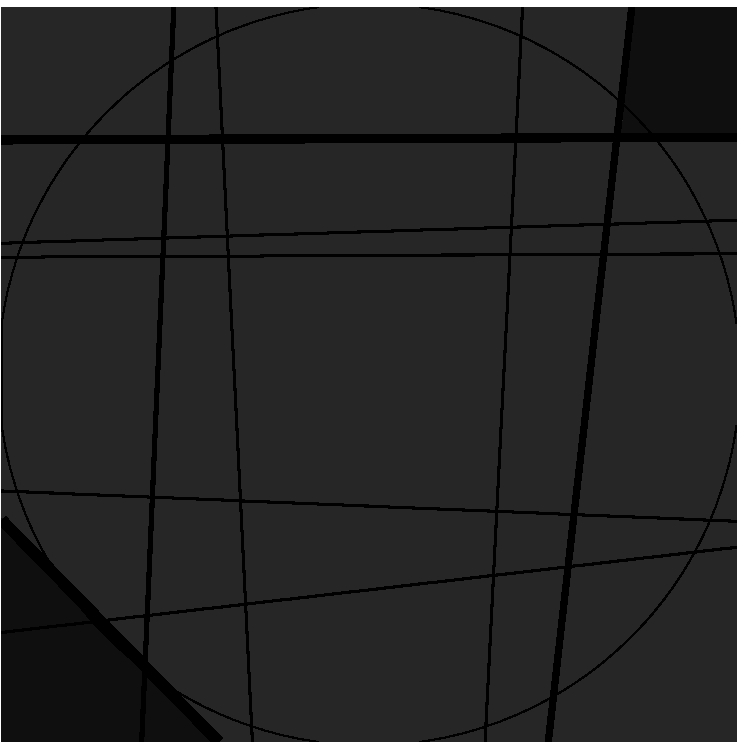
\includegraphics[scale=0.75]{big_circle.pdf}\\
Dieses Bild kommt aber auch nur zu Stande, wenn wir die Datengewichte
alle gleich initialisieren. Wenn wir sie aber so wie vorgeschlagen
initialisieren (siehe Quellcode), dann ist es ja ``nicht so schlimm''
wenn weiße Pixel falsch klassifiziert werden. Dann bekommen wir das
folgende Bild:
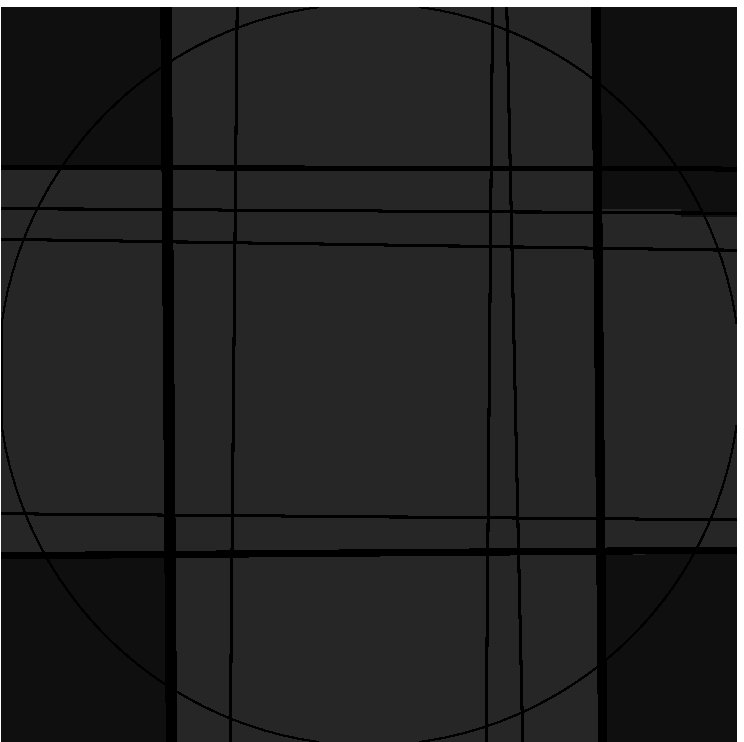
\includegraphics[scale=0.75]{big_circle2.pdf}\\
\newpage
Falls der Kreis sehr klein ist, dann verlaufen die Linien durch den
Kreis. Das kann man hier gut beobachten:\\
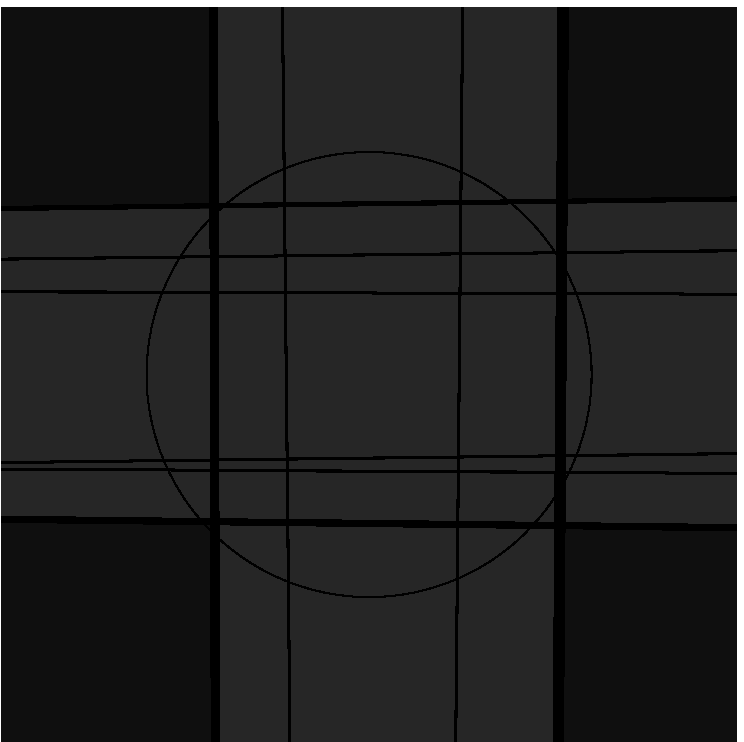
\includegraphics[scale=0.75]{03.pdf}\\


Das ergibt für uns Sinn, wenn wir uns die Fehlerfunktion und den
Algorithmus ansehen. Insbesondere kann man das bei dem folgenden Bild
nachvollziehen. Die vertikalen und horizontalen Linien, die den Kreis
schneiden klassifizieren deutlich weniger Fläche falsch, als jede
vorstellbare Tangente. Die Gewichte der Daten werden zwar ständig
angepasst, aber bis es vermeintlich endlich so weit ist, hat der
Algorithmus sehr viele schädliche Linien ausgewählt. Ansonsten konnten
wir überhaupt nicht beobachten, dass überhaupt irgendwann Tangenten
bei einem kleinen Kreis ausgewählt wurden. Entscheidend ist, dass
AdaBoost ein greedy Algorithmus ist.\\


AdaBoost ist ein greedy Algorithmus. Um ihn zu verstehen, ist es wichtig den ersten Schritt anzusehen, also die Wahl des ersten Klassifikators. In der folgenden Darstellung haben wir für einen großen und einen kleineren Kleis illustriert, warum die Tangente manchmal nicht als erstes gewählt wird. Die falsch klassifizierten Bereiche sind schwarz.\\
Beim großen Kreis (oben) ist nicht klar, ob die Wahl der Tangente besser ist als die Wahl der Gerade durch den Kreis, da die Unterschiede nur gering sind. Nur in diesem Fall haben wir Tangenten beobachtet.\\
Beim kleineren Kreis (unten) wird sichtbar, dass die Wahl der Gerade durch den Kreis die beste Wahl für den ersten Klassifikator ist. Im linken Bild sind die falsch klassifizierten schwarzen Flächen geringer als im rechten (mit der Tangente).\\
Die späteren Schritte sind sehr komplex nachzuvollziehen (aufgrund der geänderten Gewichte) und es ist nicht trivial eine Argumentation zu finden, die die Wahl von Tangenten erklären würde.\\

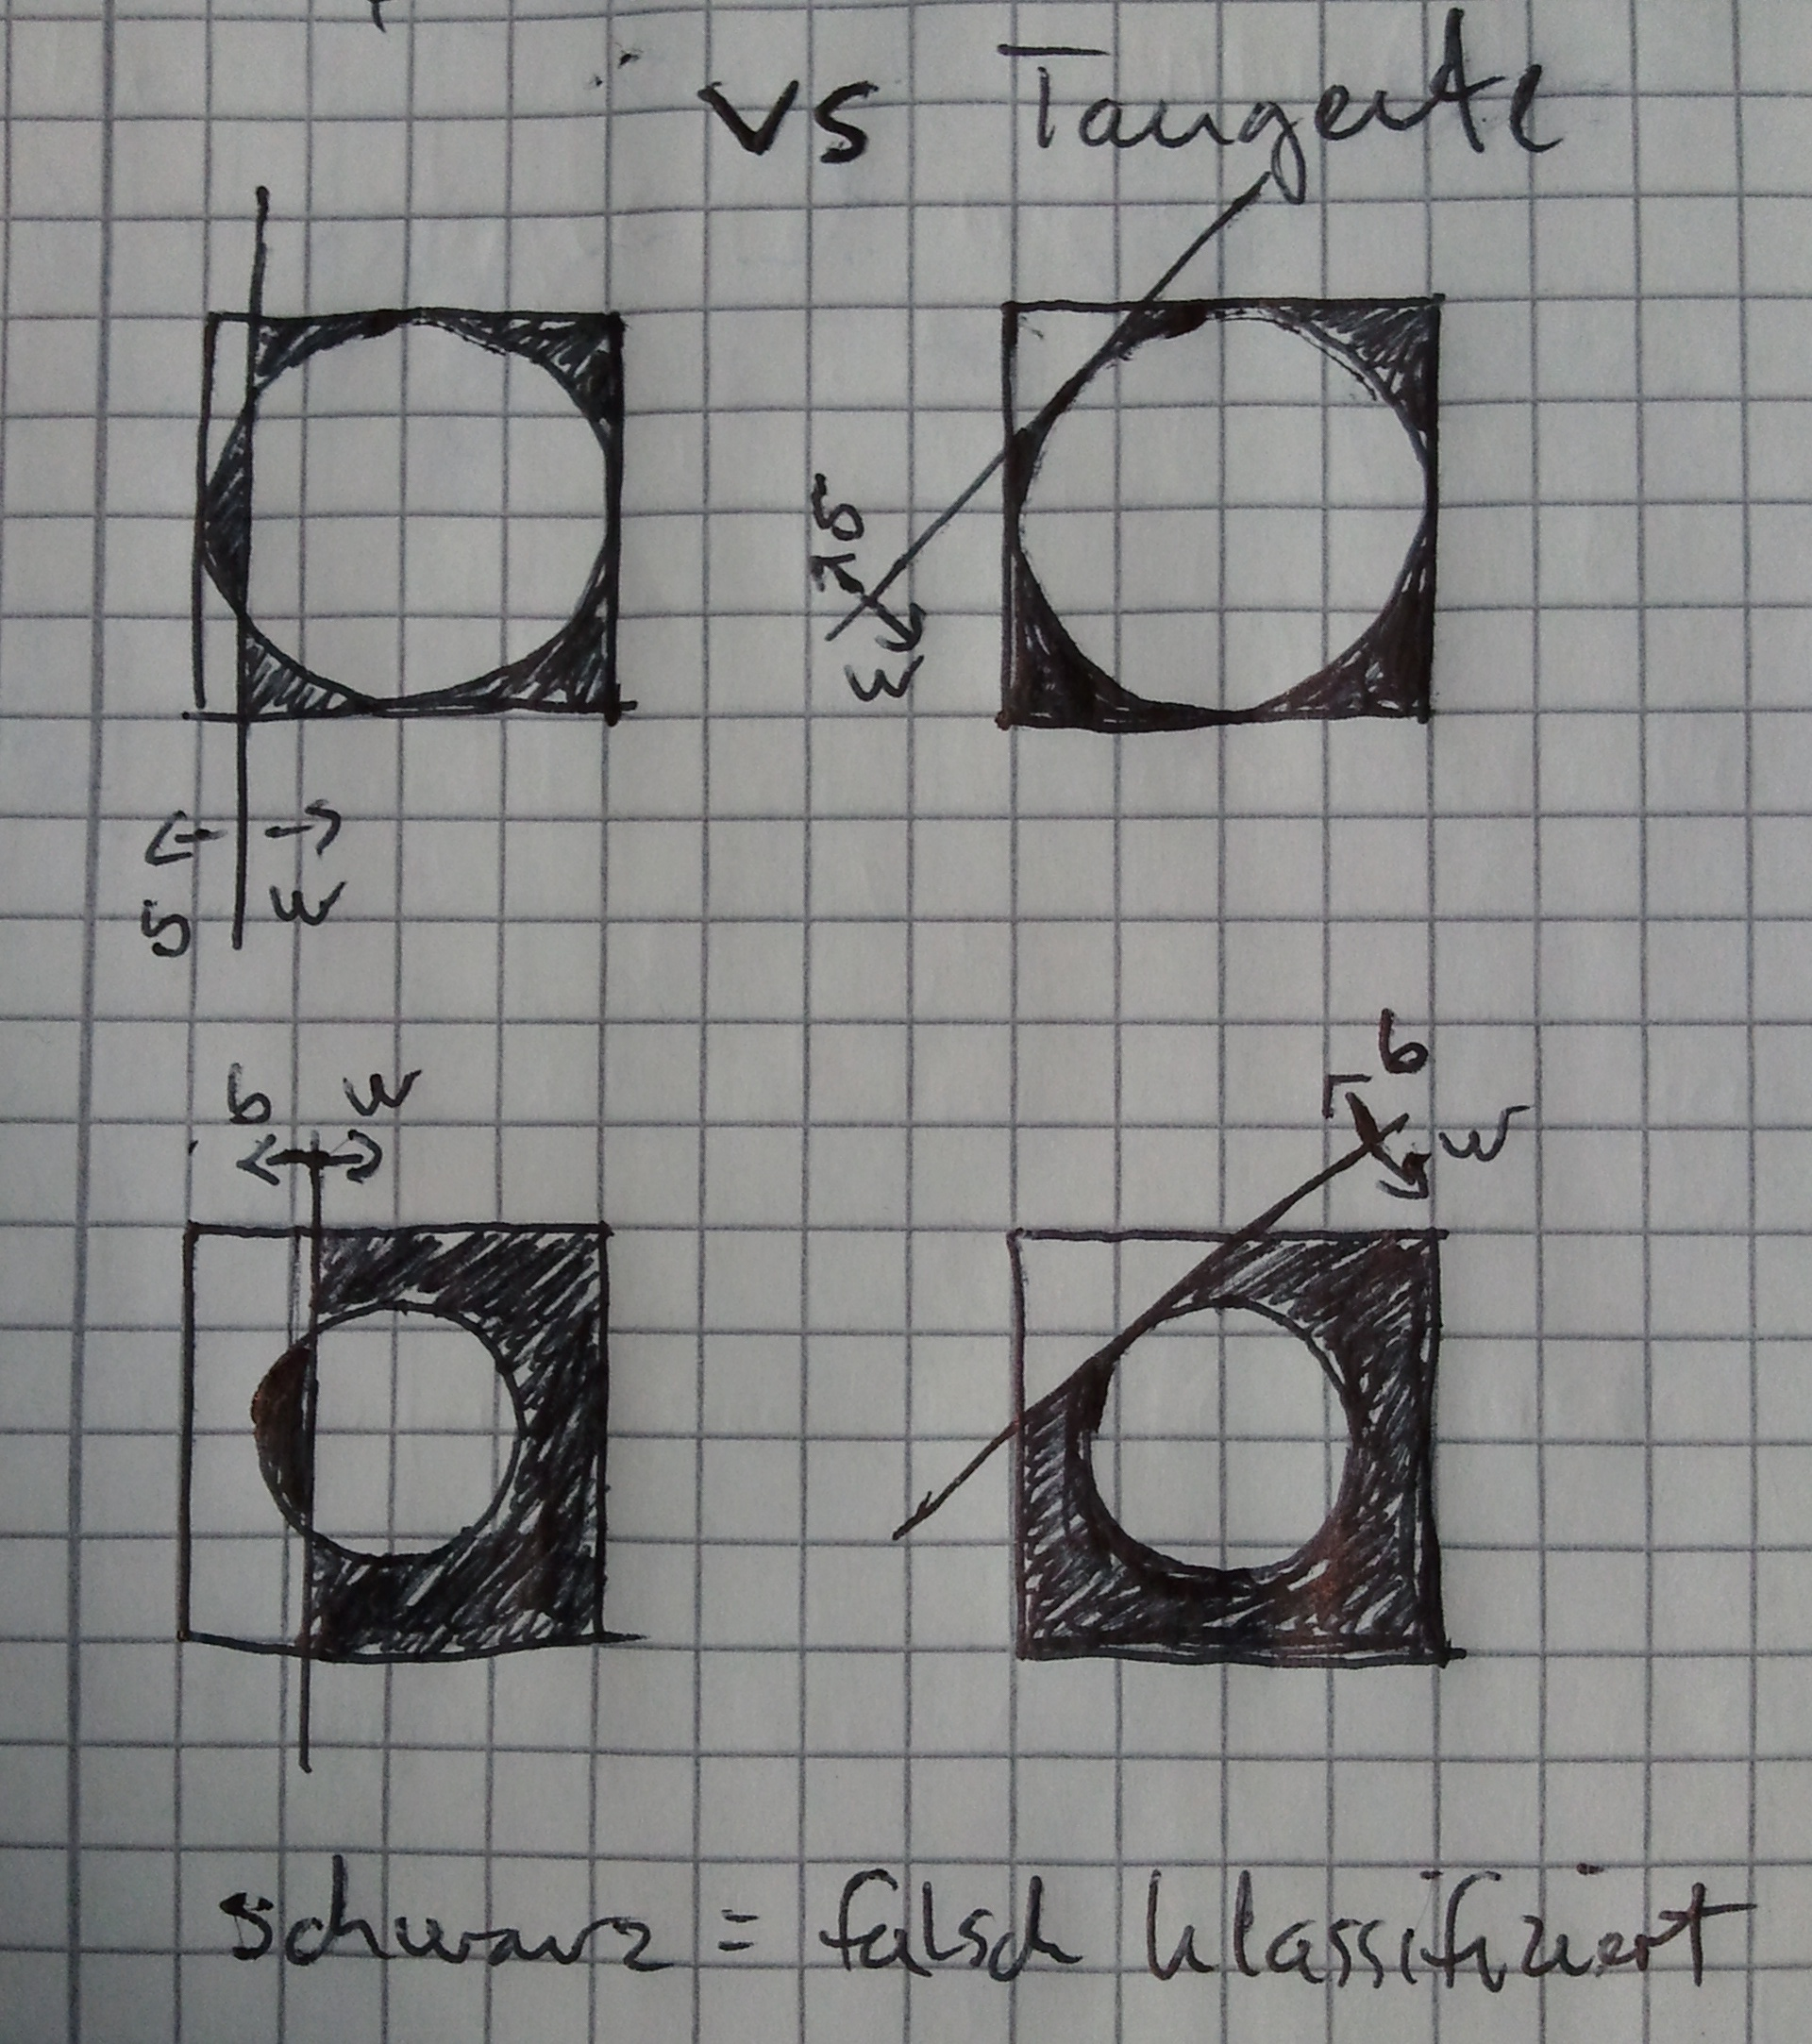
\includegraphics[scale=0.21]{zeichnung.jpg}\\




\end{document}
